\documentclass[a5paper,twoside]{scrbook}
\usepackage[ngerman]{babel}
%Schrift Quattrocento
\usepackage{quattrocento}
\usepackage[T1]{fontenc}
%Schweizer Anführungszeichen
\usepackage[german=swiss]{csquotes}
%Erlaubt Einsatz von Farbe
\usepackage{color}
%UTF 8
\usepackage[utf8]{inputenc}
%Ermöglicht Zierkapitälchen zum Anbsatzanfang
\usepackage{lettrine}
%Fourier Ornamente für Seitenkopf
\usepackage{fourier-orns}
%Ums Seitenkopf zu manipulieren
\usepackage{scrpage2} 
\pagestyle{scrheadings} 
%Auf jeder Seite ausser Kapitelanfängen oben Linie mit zwei Zeichen in der Mitte
\chead{\color{red}\hrulefill\hspace{0.2cm} \floweroneleft\floweroneright \hspace{0.2cm} \hrulefill}
%Kapitelüberschriften in Schriftart des Deckblatts
\addtokomafont{chapter}{\color{red}\rmfamily\Huge\centering\it}
%Schriftart für grosse Anfangsbuchstaben
\input Zallman.fd
\renewcommand{\LettrineFontHook}{\usefont{U}{Zallman}{xl}{n}}
%Schrift für Überschriften
\def\FontH{\fontsize{10pt}{0mm}\usefont{T1}{frc}{m}{n}}
%Grafiken einbinden
\usepackage{graphicx}
%Für Kapitel Gespenst Jonathan Rahmen ermöglichen
\usepackage[everyline=true]{mdframed}
%Definition Rahmen: links dicker roter balken
\mdfdefinestyle{mystyle}{
        roundcorner=10pt,
        backgroundcolor= red!05, 
        bottomline=false,
        rightline=false,
        linewidth=1pt,
        linecolor =red}
\mdfsetup{
%
frametitle={
%
\tikz[baseline=(current bounding box.east),
outer sep =0pt]
\node[anchor=east,rectangle,fill=red]
{\color{white} \small Olivia};},
frametitleaboveskip=\dimexpr-\ht\strutbox\relax
}

        
%Abstand zw. Wörtern darf zwecks Blocksatzbildung in Ausnahmefällen bis 1em breit werden.
\setlength{\emergencystretch}{1em}
%bessere Mikrotypographie (margin kerning insb. am Rand)
\usepackage{microtype}
%Seitenzahlen fett
\addtokomafont{pagenumber}{\bfseries}
%To-Do Kommentare einfügen -> \todo{} \missingfigure{}
\usepackage{todonotes}
% used for the 'logo'
\usepackage{tikz}            
% Totenkopf
\usepackage{skull}            
%Initialen Titelseite (Pseudologo "W")
\input Typocaps.fd
\def\FontI{\color{red}\fontsize{20pt}{0mm}\usefont{U}{Typocaps}{xl}{n}}
%%%%%%%%%%%%%%%%%%%%%%%%%%%%%%%%%%%%%%%%%%%%%%%%%%%%%%%%%%%%%%%%%%%%%%%%%%%%%%%%%%%%%%%%%%%%%%%%%%%%%%
\begin{document}
%titelseite
\begin{titlepage}
	\begin{center}
		\vspace*{3\baselineskip}
		\FontH{\Huge \color{red} Geschichten für\\ meine Töchter}\\ 
	\end{center}
		\vspace*{4\baselineskip}
	
	\begin{center}
		\begin{tabular}{p{7cm}p{5cm}}
			\textbf{\large \color{red} Gordon Wiegand} & \textbf{\large \color{red}  Linda Wiegand}\\
			\textbf{\large \color{red}\it Texte} & \textbf{\large \color{red}\it Illustrationen}\\
		\end{tabular}

	\end{center}
		\vspace*{4\baselineskip}
	\begin{center}
   		\large\FontI{W}
	\end{center}

\end{titlepage}
%Bild Seite 2
\begin{figure}[ht]
\centering
\includegraphics[width=\textwidth]{bilder/titel.jpg}
\end{figure}
%Kapitel einfügen
\chapter*{{\FontH{\Huge Flieg, Pinarella!}}\\\small \color{DeepPink} Grosi gewidmet}
\addcontentsline{toc}{chapter}{Flieg, Pinarella!}
\lettrine[lines=3]{\color{DeepPink}P}{inarella} war ein Schmetterling. Träge lag sie wie jeden Morgen auf dem Regal im Wohnzimmer der Familie Emil und liess sich die Sonne auf die Flügel scheinen. Sie gähnte, so laut das Schmetterlingsdamen eben können, und blickte sich gelangweilt im Zimmer um. Pinarella war nämlich kein einfacher Schmetterling, nein, sie bestand aus einem Körper aus Holz und die Flügel waren aus bunter Folie gemacht. Schön sah das zwar aus, aber zum Fliegen taugte so ein Körper nicht. Cornelia, die Tochter der Emils, hatte Pinarella gebastelt, als sie so ungefähr in der dritten Klasse gewesen war. Aber das war jetzt schon viele Jahre her, Cornelia hatte selbst schon zwei Kinder und mit denen war sie gerade zu Besuch bei ihren Eltern. 

Eigentlich wohnte Pinarella gar nicht auf dem Regal, sondern hing für gewöhnlich an einer Schnur über dem Ofen. Aber das letzte Mal, als Cornelia mit den Enkelinnen dagewesen war, war sie beim Spielen auf dem Boden gelandet und von da hat sie jemand auf das Regal gelegt. Bisher hatte sich noch niemand die Mühe gemacht, sie wieder aufzuhängen, aber das war Pinarella egal. Beide Orte waren genau gleich langweilig, so viel war klar. Deswegen war es auch ganz gleichgültig, wo sie gelagert wurde.

Es war natürlich nicht immer so langweilig bei den Emils. Vor allem wenn die Enkelinnen zu Besuch waren, war etwas los. Besonders Jette, die jüngste Tochter von Cornelia, spielte gerne mit dem Schmetterling. Jette war allerdings noch zu jung, um die Schönheit Pinarellas zu verstehen. Sonst würde sie wahrscheinlich nicht gar so garstig und nachlässig mit ihr umgehen. Mal wurde sie an den Flügeln gezogen, die dann umständlich von Frau Emil wieder festgeleimt werden mussten, dann wurde sie unachtsam unter einem Berg Legosteine vergraben. Und einmal wurde sie sogar mit auf die Pergola genommen und dann dort vergessen. Die ganze Nacht fror Pinarella ganz fürchtlerlich.

Jette war allerdings ein liebes Kind, das wusste Pinarella, deswegen nahm sie ihr das alles auch nicht übel. Sie war einfach noch zu jung. So viel wusste Pinarella über die Menschen: Wenn sie klein sind, überlegen sie manchmal nicht, was so alles passieren kann, wenn sie dies und jenes machen. Gerade gestern ist Jette alleine in ihr Stühlchen geklettert und dabei sehr unsanft abgestürzt. Das war ein Weinen! Und Jette hat sich selbst bestimmt nicht mit Absicht wehgetan, überlegte Pinarella, und deshalb war es wohl auch nicht böse gemeint, wenn Jette ihr mal wieder einen Fühler abgebissen hatte.

\afterpage{
\begin{figure}
    \thispagestyle{empty}
    \centering
    \includegraphics[width=\textwidth]{bilder/pinarella.pdf}
\end{figure}
\clearpage
}

An diesem Morgen war Jette wie so oft sehr früh munter geworden. Um den Papa nicht zu wecken, war Cornelia mit Jette ins Wohnzimmer gekommen. Da Jette auch in der Nacht schon mehrmals Lust gehabt hatte zu spielen, war ihre Mama noch sehr müde und wieder auf der Couch eingedöst. Jette spielte ein bisschen gelangweilt mit bunten Glasuntersetzern. 

Pinarella spienzelte vom Regal herab.  Auf dem Regal war sie jetzt zwar sicher vor Jette, aber eben auch alleine. Jette war viel zu klein, um so weit hoch zu kommen. Lieber wieder einen Flügel verlieren, dachte Pinarella, als den ganzen Tag hier zu liegen und nichts zu machen.

\enquote{Schade}, seufzte Pinarella, \enquote{wirklich schade, dass ich kein richtiger Schmetterling bin. Da wäre es ja doch viel lustiger, wenn ich ind die Welt hinaus fliegen könnte, um mit anderen Schmetterlingen zu spielen.} 

Jette blickte auf.

\enquote{Was ist denn mit dir los?}, fragte sie. Pinarella war verwirrt. Schon oft hatte sie versucht mit Menschen zu reden, aber so laut sie auch geschrien hatte, nie hat sie jemand gehört.

\enquote{Kannst Du mich verstehen?}, fragte sie daher ganz ungläubig. 

Jette nickte bloss. 

\enquote{Mir ist langweilig}, sagte Pinarella, \enquote{niemand spielt mit mir, meine Flügel sind schon voller Staub.}

\enquote{Dann komm doch hier zu mir geflogen!}, schlug Jette vor, die den Unterschied zwischen einem echten Schmetterling und einem gebastelten noch nicht so genau kannte. Und obwohl Jette das gar nicht so richtig interessierte, erklärte Pinarella ihr den Unterschied. Ihr war das nämlich wichtig. Jette verstand nicht alles, aber eines war klar: Pinarella wollte auch gerne fliegen können, um mit anderen Schmetterlingen zu spielen. Das verstand Jette sogar gut, sie spielte ja auch am liebsten mit anderen Kindern.

\enquote{Dann helfe ich Dir!}, beschloss Jette, hatte aber noch keine Ahnung, wie. Aber das ist normal bei kleinen Kindern. Die beschliessen immer Sachen, von denen sie noch nicht wissen, wie man das dann genau macht. Zuerst musste Pinarella mal von dem Regal herunter, das war offensichtlich. Das Regal war schon sehr hoch, sogar noch höher als Papa gross ist, schätzte Jette. Der konnte einen aber hoch nehmen, wenn man die Arme in die Luft streckt, Regale machen so etwas wohl aber nicht. Jette hatte bereits ein bisschen Lebenserfahrung. Und die sagte ihr auch, dass man etwas zu Hilfe nehmen musste.

Die beide sahen sich im Zimmer um, was denn diese Hilfe sein könnte. Jette hatte plötzlich eine Idee. Wenn sie mit dem Wasserhahn vom Waschbecken spielen wollte, schob sie sich immer das Schemelchen hin und stieg darauf. Für das Waschbecken war sie nämlich auch noch zu klein. Aber das Schemlechen war natürlich im Badezimmer und wenn man dort hin wollte, würde Mama bestimmt munter werden. Pinarella und jette mussten seufzen. Da bemerkte Jette den Stuhl. Sie schaute zu Pinarella, wieder zum Stuhl und versuchte abszuschätzen, ob man so zu ihr hinauf käme. So leise es einem kleinen Kind eben möglich ist, lief Jette zu dem Stuhl und schob ihn vorsichtig in Richtung Regal.

\enquote{Mach keinen Quatsch!} Mama war von dem Quietschen munter geworden, drehte sich aber zum Glück nochmals auf die Seite und schlief weiter. Jette und Pinarella hatten den Atem angehalten, den Jette mit einem lauten {\itshape Pffff.} jetzt wieder raus liess. Das war knapp. Wenn Mama gemerkt hätte, was Jette vor hatte, wäre sie bestimmt dagegen gewesen. Ganz leise kletterte Jette jetzt auf den Stuhl. Noch immer reichte sie nicht bis oben hin. Zum Glück lag da der Rückenkratzer vom Opa, den konnte sie nehmen und tatsächlich! Es klappte! Jette kam gerade so bis an das obere Ende des Regals. Sie erwischte Pinarella an einem Fühler und zog sie vom Regal herunter. 

Mit einem leisen {\itshape Plopp} landete Pinarella auf der Couch, aber zum Glück weit genug von Mama entfernt. Jette kletterte vom Stuhl herunter, was gar nicht so einfach war, nahm Pinarella, öffnete das Fenster und mit einem lauten 

\enquote{Jippie, flieg Pinarella!}, warf Jette den Holzschmetterling aus dem Fenster.

Natürlich konnte Pinarella nicht fliegen. Sie stürzte jäh ab und raste in Richtung Boden. 

\enquote{Da wird bestimmt noch mehr kaputt gehen, als nur ein Fühler.}, dachte Pinarella. Gerade in dem Moment ging die Sonne hinter den Bergen auf. Und mitten im Sturz traf Pinarella der allererste Sonnenstrahl des Tages. Sie konnte ihn auf ihren Flügeln spüren, zuckte instinktiv zusammen und da geschah es. Ihre Flügel bewegten sich! Erst langsam, dann immer schneller und noch bevor Pinarella auf dem Boden aufschlug, flog sie. Aus der Spielzeugpinarella war ein richtiger Schmetterling geworden. Höher und immer höher flog sie, fast so hoch wie das Haus und wieder runter zu dem Blumen auf der Wiese und einfach immer weiter. Jette jubelte vor Freude und Mama, die von ihrem Geschrei munter geworden war, fragte ganz verschlafen, was da los ist.

\enquote{Und nur wegen einem Schmetterling machst du so einen Lärm, dass du mich weckst?} Jette musste lächeln, Mama hatte gar nicht gemerkt, dass sie selbst den Schmetterling gebastelt hatte, der da geflogen war.\hfill {\color{DeepPink}\decofourleft}

\chapter*{\FontH{\Huge Der weisse Adler}}
\addcontentsline{toc}{chapter}{Der weisse Adler}
\lettrine[lines=3]{\color{DeepPink}J}{a}, Johann war eitel. Ihr werdet sagen,
dass das nicht gerade vorbildlich ist, aber so ganz unrecht hatte er nicht. Schön war er schon, der Johann. Denn Johann war der einzige weisse Adler weit und breit. Die anderen waren braun oder grau, wie Adler eben so sind. Auch schön, aber nicht so speziell wie Johann und oft ist es ja gerade das Spezielle, was wir als besonders schön oder manchmal auch als besonders hässlich empfinden. Und die anderen Adler mussten zugeben, dass das besonders reine Weiss seiner Federn tatsächlich sehr schön war. Und so nahm es Johann niemand übel, dass er so eitel war. 

Johann tat das aber gar nicht gut. Er wurde beinah von Tag zu Tag ein bisschen eitler. 

\enquote{Ha, ihr seht ja alle so schmutzig aus, mit euren braunen Federn, als ob ihr gerade in den Dreck gefallen wärt.}, rief er den anderen zu. Aber auch das war schon bald unter seiner Würde. Mit nach oben geschobenem Schnabel zog er seine Kreise in der Luft. Erhaben fühlte er sich und auserwählt vom Schicksal. Mit Verachtung blickte er auf die anderen Adler herab. Es dauerte nicht lange, da redete er sich sogar ein, der König der Adler zu sein. Und so benahm er sich auch.

Eigenartig war, dass die anderen Adler ihm glaubten. Sie dachten, weil Johann so Einzigartig aussah, müsse er wohl auch etwas besonderes sein. Und wer so besonders ist, ist sicher dazu bestimmt, der König zu sein. Also brachten sie ihm Mäuse, wenn er Hunger hatte und erfüllten ihm auch sonst alle Wünsche. Ein paar wenige Adler, die ihm besonders viele Mäuse brachten, standen in der Gunst von Johann weit oben. Sie bekam zur Belohnung von ihm eine weisse Feder geschenkt. Und weil Johann die nur selten verschenkte, waren diejenigen, die eine hatten, auch etwas besonderes und genossen bei den anderen Adlern hohes Ansehen. 

So ging es einige Jahr ganz gut. Johann war der König, er hatte seine treuen Freunde und konnte regieren wie er wollte. Nicht dass er das sehr ausgenutzt hätte. Eigentlich war er nur etwas faul und liess sich gerne bedienen. Hochnäsig zog er seine Kreise am Himmel.

Ein Adler-Sprichwort sagt, dass wer hoch steigt, auch tief fällt. Das habt ihr vielleicht schon einmal gehört, bei uns Menschen gibt es das ja auch. Und so erging es auch Johann. Eines Tages kam er auf die Idee, dass ein König auch einen Thron brauche. Aber was wäre denn gut genug, ein Thron für den König der Lüfte zu sein? Die Sonne war zu heiss. Der Mond war zwar schön, aber mal war er gross und rund und dann wurde er immer schmaler. Das passte Johann gar nicht und auch das blasse Gelb gefiel ihm nicht. Als einmal jemand vorgeschlagen hatte, er möge sich doch auf eine Wolke setzten, war er beleidigt.

\afterpage{
    \begin{figure}
        \thispagestyle{empty}
        \centering
        \includegraphics[width=\textwidth]{bilder/adler.pdf}
    \end{figure}
    \clearpage
}


\enquote{Die Wolken sind für den gemeinen Adler, nicht aber für ihren König.} Und so blieb nur der Regenbogen übrig. Der war aber tatsächlich besonders gut geeignet! Die herrlich leuchtenden Farben passten wunderbar zu den weissen Federn unseres Johann. 

Zufrieden mit seiner Wahl beäugte Johann den Regenbogen von allen Seiten und beschloss, dass hier sein Thron sein soll. So lud er alle Adler und auch die anderen Vögel des Himmels ein, Zeugen seiner feierlichen Thronbesteigung zu werden. Niemand traute sich die Einladung abzulehnen, immerhin war Johann ja der König. Und so putzte sich alles, was fliegen kann heraus und versammelte sich um den Regenbogen.

Johann, zufrieden so viele Bewunderer zu haben, plusterte sich nochmals gewaltig auf, flog bis an den höchsten Punkt des Regenbogens und setzte sich.

\enquote{Auf den Regenbogen setzten?}, höre ich euch fragen. Da habt ihr Recht, natürlich geht das nicht. Ein Regenbogen besteht nur aus Licht und auf Licht kann man sich nicht setzen. Ihr wisst das, aber Johann wusste das nicht! Und so plumpste er direkt durch den Regenbogen durch. Alle Adler und alle Vögel fingen an zu lachen. Und das Schlimmste war, der Regebogen hatte das weisse Federkleid unseres Johann ganz verfärbt. Hier ein roter Streifen, dort violette Tupfer und dazu überall gelbe und grüne Sprengsel. So sehr Johann auch flatterte und zappelte, die Farbe wollte nicht abgehen. Ja, wieder war Johann etwas besonderes, aber nicht mehr von der schönen Sorte.

\enquote{Hahaha, da kommt ja unser Fasnachts-Johann!}, riefen die anderen
Vögel, \enquote{Der sieht ja aus wie ein Clown.} Und dabei blieb es. Vorbei war
die Zeit vom König Johann. Niemand brachte ihm mehr Mäuse wenn er Hunger hatte,
niemand putzte sein Federkleid und bewundert wurde er auch von niemandem mehr.
Seine einstigen Freunde vermieden es, mit ihm gesehen zu werden. Die weisse
Feder, die er ihnen geschenkt hatte, versteckten sie im Wald. Keiner wollte
daran erinnert werden, einmal so einen bunten Vogel bedient zu haben. 

Und es wurde sogar immer schlimmer für ihn. Schon riefen die ersten anderen Adler:

\enquote{Hey, Fastnachst-Johann, bring uns Mäuse, wir haben Hunger.}, und fingen an, auf ihn einzupicken. Da blieb Johann nichts anderes übrig, als jetzt für die anderen Adler Mäuse zu suchen. Ein elendes Leben hatte er. Alle kommandierten ihn jetzt herum, so wie er sie einst kommandiert hatte. Das war nicht länger auszuhalten, beschloss er. Er konnte auch einfach nicht mehr. Er hatte keine Kraft mehr und es wurden zu viele Demütigungen.

Und so machte er sich auf den Weg und flog davon. Nach Norden flog er, weil ihm gerade nichts anderes einfiel. Weiter flog er und immer weiter, bloss weg von den anderen Adlern, immer höher in den Norden, wo nur Schnee und Eis sind und keine anderen Adler mehr wohnen. So kam Johann in das Reich der Schneekönigin.

Als die unseren Johann sah, freute sie sich. Denn ihr müsst wissen, dass am Nordpol -- und gerade da war unser Johann -- alles weiss ist. Überall nur Schnee und Eis. Kein Baum, kein Strauch und schon gar keine Blume oder sonst etwas, dass nicht weiss ist. Und so freute sich die Schneekönigin sehr, als unser bunter Johann geflogen kam. 

\enquote{Gute Tag, Johann}, sagte sie. Und nach einem langen Blick: 

\enquote{Wie schön Du bist.} 

\enquote{Ach, wenn es nur wahr wäre.}, seufzte Johann und erklärte: 

\enquote{Es ist noch gar nicht lange her, da war ich der Schönste Adler unter
der Sonne. Rein und weiss, gerade so wie der Schnee hier. Sogar König bin ich gewesen, weil ich so rein war. Aber ich wurde überheblich und hab nicht Recht getan. Ich bin faul geworden und habe mich füttern lassen. Und dann wollte ich zum König aller Vögel werden und vom Regenbogen aus regieren. Da bin ich gefallen. Meine Federn haben sich verfärbt wie ein Hemd beim Waschen und alle haben mich verstossen. So bin ich zu dir gekommen.}

Die Schneekönig verstand, dass Johann aufrichtig bereut hat und es ihm Leid tat, so überheblich gewesen zu sein. Da küsste sie ihn auf die Stirn. Ganz zart und vorsichtig. Hätte sie ihn mehr geküsst, wäre Johann sofort erfroren, denn alles, was die Schneekönigin berührt, wird sofort zu Eis. 

Ein eiskalter Schauer erfasste Johann. Noch nie hatte er so gefroren. Seine Flügel wurden steif und er konnte sich kaum bewegen. Die Federn wurden hart, als wären sie aus Glas. Ein paar brachen nur schon durch den Wind. Aber auch die Reste des Regenbogens in seinen Federn gefroren. Und sobald er sich ein bisschen erholt hatte und sich etwas besser bewegen konnte, fielen sie klirrend auf den kalten Boden.

Johann war glücklich. Er verbeugte sich zum Dank tief vor der Schneekönigin, breitete die Flügel aus und flog wieder zurück in den Süden. Dort lebte er von nun an als Adler unter Adlern. Weiss zwar und anders als die anderen, aber weder besser noch schlechter als sie. \hfill {\color{DeepPink}\decofourleft}

\chapter*{\FontH{\Huge }}
\lettrine[lines=2]{\color{red}A}{ls} die grosse Krähe die Menschen erschuf, lebten diese auf einer Insel mitten Meer. Alle Menschen waren glücklich. Das Meer wimmelte von Fischen, Obst und Gemüse wuchsen prächtig und ab und an liess sich auch ein Wildschwein fangen. Das waren dann immer besondere Tage. Die Menschen zogen ihre schönsten Kleider an und trafen sich auf dem Platz des einzigen Dorfes und machten Musik und sangen solange das Schwein über dem Feuer bruzelte. Krankheiten waren selten und Streit unbekannt, da alles allen gemeinsam gehörte.

Die Menschen achteten die grosse und brachten ihr jede Woche kleine Geschenke. Das waren meistens Muscheln, die die Kinder am Strand gefunden hatten oder der Zahn eines Wildschweins oder auch eine besonders schöne Blume. Dafür beschützte die Krähe die Menschen und zeigte ihnen, wie man das Feld bestellt und Häuser baut.

Karnouk war einer dieser Menschen. Er war jung und schön und wurde von allen geachtet. Er konnte schneller laufen als alle anderen und interessierte sich für alles was die Menschen damals kannten, was allerdings nicht sehr viel war. Am liebsten sass er am Strand und beobachtete die Vögel oder die Fische. Kanouk war der einzige, der wusste, wo sich die Wildschweine am Tag versteckt hielten, aber das verriet er niemanden, denn er dachte, dass die Wildschweine alleine entscheiden sollen, wann sie gefangen werden sollen.

Wie jeden Herbst kamen auch in diesem Jahr die Stürme. Gewöhnlich waren die nicht sehr stark, nur hin und wieder wurden ein paar Palmenwedel weggeblasen, mit denen die Menschen ihre Dächer bedeckten. Dieser eine Sturm war etwas schlimmer und er hielt viel länger an als sonst. Der Wind wollte für fünf Tage und fünf Nächte nicht aufhören zu blasen. Die Menschen verliessen ihre Häuser und suchten Schutz in einer Höhle. Als der Sturm sich endlich wieder gelgt hatte, kehrten sie in ihr Dorf zurück und sahen, was der Wind angerichtet hatte. Viele Dächer waren abgedeckt, aber das war nicht schlimm, das konnte schnell repariert werden. Aber es war noch etwas anderes geschehen. Hier und da sassen kleine Tiere, wie sie die Menschen bis dahin noch nicht gesehen hatten. Und da sie sie vor allem auf den abgerissen Palmenwedeln fanden, nannten sie sie Heuschrecken. 

Alle waren sich einig, dass Heuschrecken hässlich waren. 

\enquote{Das ist kein gutes Zeichen} riefen sie, \enquote{Wir haben die grosse Krähe verägert.} meinten sie. So überlegten alle, was sie wohl zu bedeuten hätten, aber da die Heuschrecken nach ein paar Tagen alle samt von den Vögeln gefressen wurden, gerieten sie bald in Vergessenheit. Nur Karnouk konnte sie nicht vergessen. Ihn quälte die Frage, wo die Heuschrecken wohl hergekommen waren. Hatte sie der Wind geboren? Das konnte er sich nicht vorstellen. Alle Tiere hatten Vater und Mutter, soweit er das beobachten konnte. 

Zehn Wochen zog er sich auf den höchten Berg zurück, und überlegte. Als er zurück kam, rief das Dorf zusammen und sagte: 

\enquote{Meine Freunde, ich habe lange darüber nachgedacht, wo die Heuschrecken wohl hergekommen sind. Ich glaube der Wind hat sie zu uns geweht, denn ihr wisst, sie waren erst nach dem schlimmen Sturm hier. Aber aus dem Wasser kommen sie nicht, denn sie sehen aus, wie unsere Käfer, sie müssen von einer anderen Insel sein.}

Da erhob sich grosses Gelächter bei den Menschen.

\enquote{Von einer anderen Insel?} riefen sie. \enquote{Schau dich doch um. Von unserem berg aus sieht man das ganze Meer und weit und breit ist nur Wasser. Die grosse Krähe hat nur das Meer und unsere Insel erschaffen, dahinter kommt nichts mehr. Und jetzt lass uns in Ruhe mit deinen dummen Ideen}

Aber Kanouk konnte nicht ruhen. Er rief nach grossen Krähe und wollte sie fragen, was das alles zu bedeuten hätte. Gab es doch noch irgendwo eine andere Insel als ihre? Kanouk war davon überzeugt, aber niemand wollte ihm glauben. Gerne wäre er losgeschwommen und hätte gesucht. Aber es stimmte ja was die Leute sagten: es war nichts zu sehen. Und Kanouk konnte keinesfalls ewig schwimmen. Er seufzte und fing wieder an zu überlegen, aber es wollte ihm nichts einfallen. Dann gab ihm die grosse Krähe ein Zeichen. Eine Kokusnuss viel von einer Palme direkt ins Meer, wurde von den Wellen erfasst und trieb hinaus ins Meer. Das war die Lösung! 

Kanouk fing an vieles auszuprobieren, die Leute wunderten sich immer mehr. Er war grosse Steine ins Wasser und bastelte riesige Schalen aus Palmenwedeln, die er auch ins Wasser setzte, bis sie untergingen. Eines Tages rannte er durch das Dorf und rief schreiend \enquote{Ich hab's, ich hab's!}

Verwundert lief das Dorf zu der Stelle am Strand, wo Kanouk in letzter Zeit gesessen und gebastelt hatte. Etwas, dass ein wenig aussah wie eine Schüssel lag mit der Öffnung nach oben im Sand. Sie war aus dem Holz der Palmen gemacht und mit dem Harz der Nadelbäume gestrichen. 

\enquote{Was soll das denn sein?} fragten sie sich und kratzen sich am Kopf. \enquote{Ich nenne es Boot,} sagte Kanouk \enquote{Und ich werde damit über das Meer reisen!}. Lachend kehrten die Menschen in ihre Häuser zurück, nur Kanouk blieb am Strand. Er hatte den Dorfbewohnern zeigen wollen, wie sein Boot fährt, aber niemand wollte zusehen. Es wurde dunkel. Kanouk war voller Wut. Er stiess die Schale ins Meer.

Und sie schwamm. Noch nie hatte kanouk sich so glücklich gefühlt. Er nahm seine Angel und sprang in die Schale. Die Strömung erfasste ihn und langsam trieb er vom Strand weg in die offene See. Wind wehte ihm durch die Haare. Die Palmen am Strand wurden aus der Ferne immer kleiner. Und so trieb Kanouk davon, um nie wieder auf seine Insel zurückzukehren.

Viele Tage lang sah Kanouk nur Wasser, so weit er blicken konnte. Er bekam Angst. Gegen den Hunger konnte er fischen, trinken konnte er das Wasser des Regens. Als er schon glaubte, nie wieder Land sehen zu werden sah Kanouk einen Raben. Der Rabe setzte sich auf den Rand von Kanouks Boot und sprach:

\enquote{Du bist der erste Mensch Deiner Insel, der dieses Land betritt. Du wirst einsam sein, aber fürchte Dich nicht, ich werde Dir helfen. Andere werden Dir folgen und dann sollt ihr dieses Land besiedeln. Es ist gross, viel grösser als Deine Insel. Seit sorgsam und schont die Pflanzen und Tiere die dort leben.}

\chapter*{\FontH{\Huge Das Gespenst Jonathan}}
\addcontentsline{toc}{chapter}{Das Gespenst Jonathan}
\begin{mdframed}[style=mystyle]
\lettrine[lines=3]{\color{DeepPink}A}{m} besten stelle ich mich erst einmal selbst vor. Ich heisse Olivia Maibaum und bin neun Jahre alt. 

Vor drei Wochen habe ich zum ersten Mal in meinem Leben ein Gespenst gesehen und zwar ein richtiges! Einmal habe ich zwar schon gedacht, dass ich eines sehe, das war dann aber doch nur die frisch gewaschene Jacke von Frau Maier, unserer Nachbarin. Der Wind hatte sie von der Leine gerissen und die ist mir dann entgegen geflogen gekommen, als ob da ein Gespenst durch die Luft schwebt. Hab ich mich damals erschrocken! Ich bin vor Schreck vom Fahrrad gestürzt und habe mir dabei die Hose zerrissen.  War das eine Aufregung und Mama wollte mir erst gar nicht glauben.

Aber das will ich hier gar nicht erzählen, die Geschichte vom richtigen Gespenst Jonathan ist viel interessanter.  Dass es Jonathan heisst, habe ich erst später erfahren. Aber ich will Euch mal die Geschichte von Anfang an erzählen.
\end{mdframed}

Mit einem lauten Krachen fällt die Rüstung von Ritter Odo von Gladez um. Die Weisse Frau von Burg Lauenstein kommt durch die Wand hinter der Rüstung geflogen und sieht sich den Haufen alten Blechs auf dem Boden an.

\enquote{Jonathan!}, ruft sie, \enquote{Komm sofort hierher!} Mit gesenktem Kopf kommt auch Jonathan durch die Wand. Jonathan ist der Sohn der Weissen Frau, die eigentlich Otilia Brigitta Walburga Peternella von Abendberg heisst. Aber alle nennen sie die Weisse Frau und das schon seit vierhundert Jahren. Sie ist nämlich ein Gespenst und die Mama von Jonathan, der natürlich auch eines ist. 

\enquote{Was soll ich nur mit Dir machen?}, seufzt die Mama. Andauernd wirft Jonathan etwas um. Er passt einfach nicht auf, wenn er zu schnell durch die Wände geflogen kommt und nicht merkt, dass in dem Raum zum Beispiel eine Vase oder ein Kleiderständer steht. Gespenster können nämlich nur durch Wände fliegen, durch andere Sachen nicht. 

\enquote{Durch Wände kannst du geh'n, anderes bleibt steh'n.} Schon mit 97 Jahren musste Jonathan diesen Spruch auswendig können, aber wirklich merken kann er ihn sich noch immer nicht. 

Und Jonathan war obendrein ein besonders schreckhaftes Gespenst. Wenn er glaubt, dass Menschen in der Nähe sind, nimmt er Reissaus und saust durch Burg Lauenstein, um sich zu verstecken. Besonders vor Kindern hat er furchtbare Angst. Die sind immer laut und frech und ärgern sich gegenseitig und ganz bestimmt auch ihn -- glaubt er jedenfalls. 

\begin{mdframed}[style=mystyle]
Burg Lauenstein müsst ihr wissen, ist eine alte Burg, die hier und da schon auseinander fällt. Sie liegt auf einem Hügel, gleich bei unserem Dorf. Lange Zeit hat niemand dort gewohnt und alle Türen waren fest verschlossen. Seit ein paar Wochen kommen aber immer wieder Handwerker und Architekten und Bauleute und sehen sich da um. Burg Lauenstein soll nämlich re-no-viert werden. Mal ehrlich, wie das Wort schon klingt. Die Burg soll ein Museum werden, in dem man so alles Mögliche ansehen kann, zum Beispiel wie die Ritter früher gelebt haben. Eine Sammlung alter Münzen soll auch kommen, da kann ich mir nichts langweiligeres vorstellen. 

Und mein Vater soll dort im Museum arbeiten. Er wird dann die Eintrittskarten verkaufen und auch sonst nach dem Rechten sehen, hat er mir erzählt. Darauf freue ich mich dann aber doch sehr. Wer hat schon einen Vater, der in einer Burg arbeitet? Und ich darf ihn dann immer besuchen kommen, das ist schon fest versprochen.
\end{mdframed}

\enquote{Du weisst ganz genau, dass wir als Gespenster immer ganz leise sein müssen. Die Menschen haben schreckliche Angst vor uns, deswegen verstecken wir uns ja in alten Burgen und Schlössern. Aber wenn Du so einen Radau machst, ist es mit dem Versteck bald vorbei.} Jonathan ist beleidigt. Meckern, meckern, meckern. Seit Tagen hat seine Mama schlechte Laune. Wahrscheinlich hat das etwas mit den Menschen zu tun, die jeden Tag kommen und hier etwas umräumen und dort etwas ausmessen. Und die tragen alle alberne gelbe Helme. Da haben die Ritter schon wesentlich schicker ausgesehen, denkt Jonathan. 

Er beschliesst der Sache auf den Grund zu gehen und sich die Menschen einmal genauer anzusehen. Dazu braucht er aber eine gute Idee, die dürfen ihn keinesfalls sehen. Er schwebt ein bisschen durch die Burg und probiert es in einer Lampe, aber wenn die angemacht wird, wird es ihm bestimmt zu heiss. Vielleicht in einer Rüstung? Gerade als er probeweise aus dem Helm heraus guckt, muss er so kräftig niesen, dass die Rüstung laut klappert. Viel zu unsicher, entscheidet er. Dann eben in die alte Truhe. Durch die Löcher, die die Holzwürmer in die Truhe gefressen haben, kann er wenigstens alles hören. So wird es gemacht. Es wird auch schon langsam Tag und bestimmt kommen die Menschen bald.  

\begin{mdframed}[style=mystyle]
Gespenster müsst ihr wissen, sind ganz besondere Wesen. Eigentlich sind sie völlig harmlos, aber irgendwann ist einmal jemand auf die Idee gekommen, dass sie vielleicht gefährlich sein könnten, wenn sie ja immer durch alle Wände fliegen können. Und da haben die Menschen angefangen, sich vor ihnen zu fürchten und sie zu vertreiben. Eigentlich haben aber die Gespenster viel mehr Angst vor Menschen. Sie können Menschen eigentlich gar nichts tun, ausser sie einmal kräftig zu erschrecken, was sie hin und wieder auch gerne machen. Aber weil sie von den Menschen verfolgt werden, haben sie angefangen, nur noch in Häusern zu wohnen, in denen keine Menschen mehr wohnen. Und das sind eben meistens alte Burgen und Schlösser.

Solche Häuser haben nämlich auch noch einen weiteren grossen Vorteil. Wisst ihr nämlich was Gespenster essen? Staub! Der weisse Staub, der sich auf Dingen absetzt, wenn man nicht putzt. Und weil in verlassenen Burgen niemand putzt, ist es für Gespenster wie im Schlaraffenland. Ich glaube, weil sie nur Staub essen, sind sie auch so weiss.

Aber Burgen haben auch einen grossen Nachteil. Sie sind ungemütlich und kosten viel Geld, wenn zum Beispiel einmal das Dach repariert werden muss. In einigen gibt es ein Restaurant oder ein Museum, aber so viele Restaurants und Museen wie es Burgen gibt, braucht kein Mensch. Die, die übrig geblieben sind, hat man einfach nicht mehr repariert und sie sind zerfallen. Das ist auch schlimm für die Gespenster die darin leben. Sie haben eigentlich nur eine Chance. Es muss jemand kommen und ihre Geschichte aufschreiben. Dann können die Gespenster für immer in der Geschichte weiter leben. Tja, aber dafür müssen sie erst einmal jemanden finden, der das macht.
\end{mdframed}

Heute darf Olivia ihren Vater zur Burg begleiten. Die Bürgermeisterin wird da sein und noch ein paar andere Leute, die sie nicht kennt. Ihr Vater ist etwas aufgeregt, da heute entschieden wird, wie es mit Burg Lauenstein und damit mit seiner Arbeit weiter gehen wird. Wie immer schütteln sich alle Erwachsenen die Hände und tätscheln Olivias Kopf, bevor endlich die schwere Tür zur Burg aufgeschlossen wird und alle hinein dürfen. Die Augen müssen sich erst an das dämmerige Licht gewöhnen. Draussen scheint die Sonne, aber hier kommt sie nicht wirklich rein.

Die Erwachsenen bleiben stehen und fangen an Dinge zu diskutieren, die Olivia nicht so genau versteht. 

\enquote{Herr Maibaum, ihre erste Aufgabe wird wohl sein, hier einmal richtig aufzuräumen und den ganzen Staub und Dreck zu entfernen. Dann kommen Frau Doktor Hampel und Herr Doktor Wagner von der Universität und gemeinsam werden Sie eine Liste all der Sachen erstellen, die es hier gibt.} hört Olivia die Bürgermeisterin zu Ihrem Vater sagen, dann ist es ihr schon zu langweilig und sie fängt an, sich selbst etwas umzusehen.

All die Rittersachen mag sie nicht, dass merkt sie schnell. Schwerter sind dafür da gewesen, andere umzubringen, die findet sie blöd. Und als sie die Rüstungen sieht, überlegt sie, ob es nicht schrecklich unbequem gewesen sein muss, so ein Ding anzuhaben. 

Eine Maus läuft direkt auf sie zu. Die scheint gar keine Angst zu haben. Olivia lacht und sagt:

\afterpage{
    \begin{figure}
        \thispagestyle{empty}
        \centering
        \includegraphics[width=\textwidth]{bilder/gespenst1.pdf}
    \end{figure}
    \clearpage
}
\enquote{Du bist viel mutiger als die Ritter in ihren Blechrüstungen.} So mutig ist die Maus aber doch nicht und verschwindet im Dunkeln. Olivia versucht hinterher zu rennen, aber plötzlich fällt ihr Blick auf eine grosse, schwere Truhe. Ihre Augen glänzen. So eine hat sie schon einmal in ihrem Buch mit Piratengeschichten gesehen. Da war dann ein unglaublicher Schatz in der Truhe. Ob hier wohl auch einer drinnen ist? Sie versucht den schweren Deckel hoch zu heben, aber das klappt nicht. Viel zu schwer. 

Herr Wagner, der später ihrem Vater helfen soll, kann sofort erraten, was sie da macht. 

\enquote{Na, suchst Du Schätze?}, will er wissen. Olivia fühlt sich ertappt und weiss nicht was sie sagen soll. Aber Herr Wagner lächelt, er scheint also nicht böse zu sein. Erwachsene sind ja schnell mal böse, wenn Kinder nicht genau das machen, was man ihnen gesagt hat. Olivia hat noch nicht ganz genau durchschaut, was man jetzt darf und was nicht und schon gar nicht, wenn es darum geht, Schätze in alten Burgen zu suchen.

\enquote{Warte, ich helfe Dir.} sagt er. Nett, denkt Olivia. Zusammen versuchen sie den Deckel zu heben, aber wieder klappt es nicht. Herr Wagner fängt an das Schloss zu untersuchen und runzelt die Stirn.

\enquote{Also verschlossen ist die Truhe nicht. Die klemmt, das kann bei so alten Truhen schon mal vorkommen.} Später kommen noch die Bürgermeisterin und andere Erwachsene hinzu und versuchen die Truhe zu öffnen, aber alle scheitern. Herr Wagner entscheidet, dass die Truhe als erstes aus der Burg geschafft werden soll und zwar direkt in die Werkstatt zu den Maibaums, damit er sie untersuchen kann.

\enquote{Vielleicht ist ja wirklich ein Schatz darin versteckt. Übermorgen komme ich und dann sehen wir uns das gemeinsam an.}, sagt er und zwinkert Olivia zu. 

Was keiner der Anwesenden ahnt, ist das die Truhe keineswegs klemmt. Und ein Schatz befindet sich auch nicht darin, sondern das kleine und sehr verängstigte Gespenst Jonathan. Der weiss vor lauter Angst gar nicht was er machen soll und hält den Deckel so fest zu wie er kann. Als Herr Maibaum und Herr Wagner die Truhe unter Schnaufen und Prusten hoch heben und auf ein Auto verladen, wird er fast ohnmächtig vor Angst. Was werden die wohl mit ihm machen?

Beim Abendessen ist Vater Maibaum sehr aufgeregt und erzählt seiner Frau in allen kleinen Details, was wer gesagt hat und wie wer dabei geguckt hat. Das ist schon an normalen Tagen furchtbar langweilig für Olivia, aber heute ganz besonders. Erstens ist sie dabei gewesen und weiss das alles schon und zweitens will sie doch unbedingt nochmals in die Werkstatt und sich die Truhe ansehen. 

Sie hat nämlich in Ihrem Piratenbuch nachgesehen. Da haben sie die Schatztruhe auch erst nicht auf bekommen, es dann aber mit einer Eisenstange geschafft. Wie genau weiss Olivia auch nicht, aber sie will es unbedingt noch heute versuchen. Als sie endlich vom Tisch aufstehen darf rennt sie sofort in die Werkstatt. Sie nimmt ein langes Rohr, das in der Werkstatt an der Wand steht und nähert sich der Truhe.

Das ist genau der Augenblick, als Jonathan es nicht mehr aushält und den Deckel vorsichtig öffnet, um mal einen Blick ins Freie zu werfen. Er blickt durch den sich öffnenden Spalt und sieht wie ausgerechnet ein Kind, eines dieser gefährlichen Schreihälse, mit einer Stange bewaffnet auf ihn zu kommt. Das ist zu viel für ihn. Er schreit wie er noch nie im Leben geschriehen hat.

\begin{mdframed}[style=mystyle]
  Ihr könnt euch vorstellen, dass es mir nicht viel anders erging als Jonathan. Als sich plötzlich der Deckel wie von alleine geöffnet hat und ein echtes Gespenst zu sehen war, das auch noch angefangen hat zu schreien wie verrückt, habe ich vor Schreck die Stange fallen lassen. Das hat einen so lauten Knall gegeben, dass sofort Papa in die Werkstatt gestürzt gekommen ist, und wissen wollte, was los ist. Ohne meine Antwort abzuwarten hat er gleich geschimpft und gemeint, die Kiste dürfe ich nicht anfassen, die sei alt und \emph{wissenschaftlich wertvoll}, wie er das mit wichtiger Mine genannt hat. Da dürfe nichts kaputt gehen, nicht einmal ein kleiner Kratzer sei erlaubt. Dabei ist die Kiste doch uralt und schon von alleine ganz wurmstichig. 
  
Verstanden habe ich das nicht. Aber ich musste sofort ins Bett. Da habe ich es natürlich nicht ausgehalten. Als Mama und Papa endlich wie jeden Abend vor dem Fernseher eingeschlafen waren, bin ich sofort wieder in die Werkstatt geschlichen. Zweimal tief Luft holen musste ich schon. Immerhin war ja ein Gespenst in der Werkstatt. Ich habe all meinen Mut zusammen genommen und habe die Tür geöffnet. Jonathan sass zitternd in der Ecke, weswegen ich plötzlich keine Angst mehr hatte. 
\end{mdframed}

Olivia geht langsam auf das Gespenst zu. 

\enquote{Ich heisse Olivia und wer bist Du?} fragt sie. Jonathan bekommt erst kein Wort heraus, merkt aber auch schnell, dass das Mädchen wohl doch nicht so gefährlich ist, wie er erst dachte. Erst sagt er nur seinen Namen, aber dann sprudelt es aus ihm heraus. Dass er ein Gespenst sei, erzählt er -- als ob Olivia das noch nicht gemerkt hätte -- und dass er auf Burg Lauenstein wohne, seine Mutter die Weisse Frau sei, dass er Angst vor Kindern habe, aber eigentlich noch nie eines kennengelernt hat und noch ein paar andere Dinge mehr. 

Olivia will natürlich auch gleich vieles wissen. Wie es ist, ein Gespenst zu sein und ob man als Gespenst zum Beispiel zaubern kann. Kann man allerdings nicht. Na ja, nicht wirklich zaubern, aber immerhin durch Wände gehen und das beeindruckt Olivia dann natürlich sehr. Immer wieder muss Jonathan durch die Werkstatt fliegen, durch die eine Wand raus durch die andere wieder rein, mal nur mit dem Kopf aus der Wand gucken und Grimassen schneiden. 

\enquote{Ich habe Hunger, willst Du auch was?}, ruft Olivia und ohne eine Antwort abzuwarten saust sie in die Küche. Als sie am Wohnzimmer vorbei muss, zieht sie ihre Schuhe aus, damit es keinen Ton gibt und Mama und Papa munter werden. Mit Schokoriegeln in der Hand kommt sie zurück. Jonathan stutzt und meint, dass er als Gespenst natürlich nur alten Staub zum Essen mag und Schokoriegel ganz unter seiner Würde seien. Olivia ist zwar verblüfft, aber dann bleibt eben mehr für sie übrig. Und Staub gibt es in der Werkstatt mehr als zehn Gespenster in einem Jahr schaffen würden.

\enquote{Was haben eigentlich die vielen Leute heute bei uns in der Burg gemacht?}, will Jonathan schmatzend wissen.

\enquote{Die haben sich angesehen, wie die Burg neu umgebaut werden soll. In ein Museum. Und mein Vater hilft auch mit und muss als erstes putzen. Schon in einer Woche geht es los.}, weiss Olivia. Jonathan muss sich vor Schreck fast verschlucken.

\enquote{Aber dann haben wir ja gar nichts mehr zum Essen. Und wo sollen wir dann wohnen?}, ruft er aufgeregt. \enquote{Dass muss ich sofort Mama erzählen.} Und schon fliegt er los.

\enquote{Aber komm mich doch mal wieder besuchen!}, kann Olivia ihm gerade noch hinterher rufen.

Schon am nächsten Tag kommt Jonathan zurück. Und mit ihm seine Mutter, die Weisse Frau. Es war schon dunkel und Olivia wollte sich gerade hinlegen, als es am Fenster klopft. Sie dachte sich zwar schon, wer das sein könnte, aber zur Sicheherheit nimmt sie ihren Teddy als Beschützer unter dem Arm mit. Sie bekommt dann doch einen Schrecken, als sie die Weisse Frau sieht. So ein ausgewachsenes Gespenst ist dann schon noch etwas anderes, als ein Kindergespenst. Olivia muss nochmals genau erzählen, was sie auf der Burg mitbekommen hat, als die Bürgermeisterin geredet hat.

Die Weisse Frau hört sich das alles an und fragt hier und da nochmals nach und sagt dann: 

\enquote{Da hilft alles nichts.}, und streichelt dabei Jonathan über den Kopf, \enquote{Wir müssen umziehen.} Aber wohin? Keiner der Drei kennt eine leer stehende Burg. Olivia schaltet den Computer an und sucht im Internet.

\enquote{Nein, nichts.}, sagt sie. Die einzige leere Burg, die sie finden kann, ist eine Ruine, aber die ist schon sehr zerfallen. Von der stehen nur noch ein paar Mauerreste. Alle seufzen. Aber die Weisse Frau ist schon ein altes Gespenst und weiss einen Rat.


\begin{mdframed}[style=mystyle]
Und der Rat der Weissen Frau war, dass auch sie beide das machen müssen, was schon so viele Gespenster vor ihnen getan haben. Sie müssen nicht in eine andere Burg umziehen, sondern zu einer Geschichte werden. Über die weisse Frau gibt es schon viele Geschichten. Aber über Jonathan bisher noch keine einzige. Und deswegen bin ich von den beiden gebeten worden, die Geschichte aufzuschreiben, wie ich Jonathan kennen gelernt habe. Und das habe ich ja jetzt getan. Jonathan wohnt hier in dieser Geschichte, die ich euch gerade erzählt habe. 

Aber Vorsicht! Jeden, der die Geschichte hört, kommt Jonathan mindestens einmal besuchen. Er ist aber immer noch sehr ängstlich. Er versteckt sich dann irgendwo bei euch. Und wenn ihr es schon bald mal irgendwo klappern hört und ihr wisst nicht warum, dann war das bestimmt Jonathan. Und wenn mal ein Spielzeug von euch fehlt, dürft ihr auch nicht böse sein. Das hat sich dann Jonathan geborgt. Immer in derselben Geschichte zu wohnen, ist ja auch etwas langweilig. Aber er hat mir ganz fest versprochen, dass er euch euer Spielzeug immer schon bald zurückbringt. Aber seid so nett und putzt nicht immer so fest! Wenn Jonathan kommt, freut er sich immer, hier und da mal ein bisschen Staub naschen zu können. \hfill {\color{DeepPink}\decofourleft}
\end{mdframed}


\chapter*{\FontH{\Huge Der Fall der verschwundenen Schmetterlinge}}
\addcontentsline{toc}{chapter}{Der Fall der verschwundenen Schmetterlinge}
\lettrine[lines=3]{\color{red}D}{as} Mobiltelefon klingelt weckt und Fenja aus dem Schlaf. Es ist noch sehr früh am Morgen. Zuerst bemerkt Fenja, dass es noch gar nicht hell ist. Eine Frechheit, wer ruft sie so früh an? Am Klingelton erkennt sie sofort, dass es Kommissarin Bettina Andermatt sein muss.

Sofort ist sie hellwach. Fenja geht zwar noch in die Schule, aber sie ist sehr intelligent und kann auch sonst noch viele Dinge besser als andere Menschen, sogar besser als die meisten Erwachsenen. Deswegen bittet sie die Polizei regelmässig, bei der Aufklärung von Verbrechen zu helfen. Es scheint wieder einmal soweit zu sein.

\enquote{Ja, aha, ich verstehe.} Fenja schreibt alles, was die Kommissarin sagt in ein kleines Notizbuch, dass immer auf ihrem Nachtschränkchen liegt. Im Papillorama in Kerzers sind Schmetterlinge verschwunden. Seltene, besonders schöne Exemplare der Gattungen \emph{Morpho peleides}.

\enquote{Entschuldigen sie die Frage, Frau Kommissarin, aber könnte es sein, dass die Schmetterlinge einfach abgehauen sind? Ich selbst würde auch jede Gelegenheit nutzen, wenn ich so eingesperrt wäre.} Im Zimmer kann man hören, wie die Kommissarin am anderen Ende der Leitung lauter wird. Für vorlaute Spässe hat sie keinen Sinn, schon gar nicht um diese Uhrzeit. Sie erklärt, dass es auffällig ist, dass nur Schmetterlinge eben jener Sorte verschwunden sind. Ausserdem sind auch alle Raupen weg.

Fenja verspricht der Sache sofort am nächsten Morgen nachzugehen und legt auf. Zunächst müssen die organisatorieschen Dinge geklärt werden. Das Papilorama liegt in Kerzers, das weiss Fenja aber schon. Der erste Zug geht 7:32\,Uhr. Jetzt ist es 4:35\,Uhr. Genügend Zeit, sich vorzubereiten. Folgende Dinge kann Fenja mit Hilfe des Internet recherchieren:

\begin{description}
	\item[Morpho peleides] \sffamily{Deutsch: Blauer Morphofalter. Der Schmetterling gehört zur Familie der Edelfalter. Die Flügel haben blaue Oberseiten und können eine Spannweite bis 12\,cm haben. Sie ernähren sich von faulenden Früchten.}
\end{description}

Fenja staunt. So riesige Schmetterlinge hat sie noch nie gesehen. Mit Hilfe des Lineals macht sie in ihrem Notitzheft ein Quadrat mit einer Höhe und Breite von zwölf Zentimetern und zeichnet einen Schmetterling. Den malt sie blau aus. 

Dann beginnt sie ihren Rucksack zu packen. Sie benötigt:

\begin{enumerate}
  \item Die Detektivausrüstung bestehend aus ein paar sauberen Handschuhen, einer Lupe, einer Pinzette und ein paar leeren kleinen Tüten.
  \item Etwas zum Essen und zum Trinken.
  \item Regenjacke
  \item Etwas Geld
\end{enumerate}

Das alles passt wunderbar in ihren Rucksack. Noch die Schuhe und dann\dots steht plötzlich Carla, ihre kleine Schwester vor ihr. Die wacht immer sehr früh auf und scheint etwas bemerkt zu haben. Carla ist zwar noch ziemlich klein, aber auch nicht dumm. Sofort begreift sie, dass Fenja irgendwo hin will. Und sie weiss genau, dass es mit ihrer grossen Schwester oft aufregende Dinge zu erleben gibt.

\enquote{Wenn Du mich nicht mit nimmst, fange ich so laut an zu weinen, dass Mama und Papa aufstehen.}

Das hätte gerade noch gefehlt. Die wollen nämlich eigentlich nicht, dass Fenja der Polizei hilft. Viel zu gefährlich meinen sie. Lächerlich. 

\enquote{Was willst du?} fragt Fenja. \enquote{Wenn Du leise bist, erlaube ich Dir so viele Trickfilme auf meinem Computer zu sehen, wie du willst.} Das ist zwar tatsächlich das verführerischste Angebot, dass die grosse Schwester machen kann, aber Carla lässt sich nicht beirren.

\enquote{Auf gar keinen Fall! Ich will mit!} Fenja seufzt. Aber sie wäre nicht sie selbst, wenn sie nicht auch aus dieser Situation das Beste machen könnte. Sie nimmt Carla mit. Das ist die beste Tarnung. Jetzt in den Ferien sind viele Kinder im Papiliorama, da fallen sie beide gar nicht auf und können sich in Ruhe umsehen.

Der Zug erreicht Kerzers pünktlich. Auf dem Weg zum Papiliorama erklärt Fenja ihrer Schwester was passiert ist. Sie schärft ihrer Schwester ein, dass sie nicht zum Spass hier sind. Die Schmetterlinge kann man sich auch ein anderes Mal noch ansehen. Jetzt heisst es ermitteln und Spuren sammeln.

Der Direktor des Papilioramas, Herr Butterblom, weiss, dass Fenja kommen wird. Kommissarin Andermatt hat ihn schon informiert. Die beiden Schwestern wollen getrennt ins Papiliorama gehen und sich in einer Stunde in der Cafeteria bei den Süssigkeiten treffen. Niemand wird glauben, dass Carla auch ermittelt.

Fenja hat sich überlegt, dass es sich bei den Dieben der Schmetterlinge nur Menschen handeln kann, die sich auf irgendeine Art für Schmetterlinge interessieren. Denn wertvoll sind sie nicht. 

\enquote{Herr Butterblom, wer könnte ein Interesse an diesen Schmetterlingen haben?} Fenja weiss, welche Fragen als erstes gestellt werden müssen. Herr Butterblom überlegt.

\enquote{Das weiss ich auch nicht. Es gibt natürlich Leute, die sich für Schmetterlinge interessieren und die selber züchten. Und da kommt es schon einmal vor, dass die hier ein paar Raupen klauen. Aber gleich alle ist noch nie passiert.} 

\enquote{Kennen sie diese Sammler? Können sie mir vielleicht die Liste aller Namen geben?} will Fenja wissen.

\enquote{Natürlich nicht.} antwortet Herr Butterblom. Was für eine Frage. Woher soll er denn die Namen der Leute kennen, die Schmetterlinge züchten? Aber Fenja ist etwas schlauer als er.

\enquote{Auf ihrer Web-Seite habe ich gesehen, dass sie auch Tagungen zu Schmetterlingen organisieren. Beispielsweise hat gerade letzte Woche jemand von der Universität einen Vortrag zu Schmetterlingen in den Alpen gehalten.} Fenja ist wirklich sehr gut vorbereitet. \enquote{Ich denke, dass alle, die sich für Schmetterlinge interessieren, auch an solchen Veranstaltungen teilnehmen. Es wäre sehr hilfreich, wenn sie mit die Anmeldelisten der letzten beide Jahre per E-Mail schicken könnten.}

Herr Butterblom ist verblüfft. Tatsächlich. Wenn es Züchter gibt, dann kommen die auch hierher und bei Veranstaltungen muss man immer vorher seinen Namen nennen, damit man reservieren kann. 
\begin{center}
\aldineleft
\end{center}

Zur selben Zeit schlendert Carla durch die Gänge des Papilioramas. Es ist gerade eine Sonderausstellung zum Thema \emph{Schmetterlinge in der Kunst}. Künstlerinnen und Künstler aus der Umgebung wurden eingeladen, ihre Sicht auf Schmetterlingen zu zeigen. Jemand hat einen grossen Schmetterling aus Stahl geschweisst, das ist das auffälligste Ausstellungsstück. Daneben gibt es ein paar Bilder an der Wand und eine Designerin hat sogar Kleidungsstücke mit Schmetterlingen bedruckt. Carla fotografiert alles sorgfältig mit der Kamera ihres Telefons.

\enquote{Alles grosser Unfug} hört Carla neben sich sagen. Eine gross gewachsene Frau mit einem sehr eigenartigen Hut blickt verächtlich auf die ausgestellten Dinge. Carla fragt:

\enquote{Ihnen gefallen die Bilder wohl nicht besonders?}

\enquote{Natürlich nicht.} ruft die Frau mit sich überschlagender Stimme. \enquote{Das ist doch alles Unfug. Neben der Schönheit der Farben eines echten Schmetterlings, ist das hier alles blass und langweilig.} Und dann ergänzt sie:

\enquote{Darf ich mich übrigens vorstellen? Mein Name ist Verena Studer-Matt und das Kleid dahinten} dabei deutet sie auf die schmetterlingsgemusterten Kleider \enquote{sind übrigens von mir entworfen. Aber auch die finde ich mittlerweile ganz grauenvoll. Wer einmal die Schönheit eines Blauen Morphos gesehen hat, ist für derartiges verloren.} 

%\begin{figure}[h]
%\centering
%\includegraphics[width=.7\textwidth]{bilder/kerzers.pdf}
%\end{figure}

Mit einer Miene, die tiefen Ekel ausdrücken soll und ohne eine Antwort von Carla zu erwarten stapft die Dame davon. Ob sie weiss, dass gerade diese Schmetterlinge alle verschwunden sind, überlegt Carla.

Die beiden Schwestern treffen sich in der Cafeteria. Wie immer darf sich Carla nichts kaufen sondern muss das essen, was Fenja mitgebracht hat. Fenja erzählt kauend, dass man als nächstes bei den Sammlern und Züchtern nachfragen muss. Es sind im Moment die einzigen Verdächtigen. Und weil es klar ist, dass sie hier nicht weiterkommen, beschliessen sie nach Bern zu fahren, an der Universität gibt es einen Spezialisten für Schmetterlinge. Das ist der, der neulich hier den Vortrag gehalten hat, am besten man fängt bei dem gleich an. Vielleicht hat der eine Ahnung, wer wohl ein Motiv hat, Schmetterlinge zu stehlen.
\begin{center}
\aldineleft
\end{center}

 Als sie in Bern ankommen, hat Fenja schon über das Internet herausgefunden, wie sie zur Universität kommen und wo sie dort den Schmetterlingsexperten finden. Dr.\,Carlos Moreira heisst er, das Büro von ihm müssen sie jetzt suchen. \emph{Zoologisches Institut} steht über der Eingangstür. Als ob Fenja jeden Tag hier wäre, geht sie zielsicher zum Fahrstuhl und drückt den Knopf zum dritten Stock. Woher ihre Schwester wohl immer so genau weiss was zu tun ist, überlegt Carla.

\enquote{Hallo ich bin Carlos} begrüsst sie ein junger Mann mit stark spanischem Akzent. Das verblüfft dann sogar Fenja. Sie hätte sich Professoren viel älter vorgestellt und das sagt sie ihm auch, um sicher zu gehen, dass sie mit dem richtigen spricht. Carlos muss lachen. \enquote{Na erstens bin ich noch kein Professor und ausserdem seid ihr beiden ja auch nicht im typischen Alter von Detektivinnen seid.} Er schiebt den beiden je eine Dose Cola hin. Zu Hause dürfen sie die nie trinken, was aber natürlich keine der beiden stört. Nichts anmerken lassen, heisst es jetzt.

\enquote{Also, wie kann ich Euch helfen?} Fenja erklärt was passiert ist. Carlos hört sehr aufmerksam zu.

\enquote{Nein. Da kann ich euch nicht helfen. Ich habe keine Ahnung, wer so etwas tun könnte. Aber halt, wartet einmal. neulich war eine Dame hier, die hat sich genau für diesen Schmetterling interessiert. Und die wollte wissen, wie man es am besten schafft, dass die Flügel auch nach dem Tod der Schmetterlinge möglichst lange halten und ihr Blau behalten.}

\enquote{Wie heisst die Frau?} Fenja ist wie elektrisiert. Das ist die erste echte Spur. So etwas kann kein Zufall sein. Carlos überlegt und schaut in seinem Computer nach.

\enquote{Ich befürchte, dass ich den nicht kenne. Ich glaube, die hat sich gar nie richtig vorgestellt. Aber ich kann sie euch beschreiben. Sie ist schon etwas älter, gross und wenn ihr mich fragt\dots} und an statt etwas zu sagen tippt er sich mit dem Finger an die Stirn \enquote{Na jedenfalls hatte sie einen wirklich exzentrischen Hut auf. Riesig und mit Federn.} jetzt ist Carla aufgeregt. 

\enquote{Die habe ich heute gesehen, im Papliliorama. Das ist die Frau, die die Kleider mit dem Schmetterlingsmuster gemacht hat!} Carlos und Fenja sehen Carla verblüfft an. Carla erinnert sich, dass die Frau auch ihren Namen genannt hatte, aber den hat sie lengst vergessen. Namen kann sie sich einfach nicht merken. Und bevor Fenja böse ist, sagt sie lieber nicht, dass sie den Namen kennen sollte.

\enquote{Wie die heisst, weiss ich auch nicht, aber ich habe die Kleider fotografiert.} Carlos und Carla blicken auf das Display von Carlas Telefon. Fenja ruft derweil Herrn Butterblom an. Der weiss den Namen auch nicht auswendig, sieht aber schnell auf dem Schild unter dem ausgestellten Kleid nach. Studer-Matt heisst sie.

\enquote{Richtig}, ruft Carla, \enquote{jetzt fällt es mir auch wieder ein.} Fenja runzelt mit Blick auf ihre Schwester die Augenbrauen und schlägt aber ohen etwas zu sagen im Telefonbuch die Adresse nach. Mit kleinen Schwestern zu schimpfen lohnt sich nicht und den Namen haben sie ja jetzt auch so.

\enquote{Na ich komme mal besser mit.} sagt Carlos.

Als sie bei Frau Studer-Matt ankommen, riecht es sehr verfault. Carlos will an der Tür klingeln.

\enquote{Halt!} ruft Fenja. \enquote{Wenn die Schmetterlinge da drin sind, ist es besser wenn die Tür geschlossen bleibt. Die Schmetterlinge leben eigentlich in tropischen, also warmen Gebieten. Kalter Wind ist schädlich. Im Übrigen bin ich der Meinung, dass die Schmetterlinge sicher hier sind. Richt ihr nicht den Geruch? Das ist faulendes Obst, das Lieblingsessen des Blauen Morphofalters. Ich rufe jetzt Kommissarin Andermatt an, wir warten hier so lange.}

Carlos ist verblüfft. Das hätte er eigentlich alles selber merken können. Hat er aber nicht. Eine halbe Stunde später ist die Kommisarin da. Sie hat auch gleich noch ein paar Kollegen mit gebracht, als Verstärkung. Sie klingeln jetzt doch an der Tür. Eine genervte Frau, die ganz offensichtlich tatsächlich Frau Studer-Matt ist, öffnet die Tür. Und auf ihrer Schulter sitzt auch schon der erste blaue Schmetterling.
\begin{center}
\aldineleft
\end{center}

Die Polizisten nehmen Frau Studer-Matt mit auf das Polizeirevier. Carlos und Herr Butterblom fangen so lange die Schmetterlinge in der Wohnung ein und bringen sie zurück ins Papiliorama. 

\enquote{Warum haben sie das getan?} Kommissarin Andermatt spricht die Frage aus, die alle brennend interessiert.

\enquote{Ich wollte, ich, \dots} Frau Studer-Matt kommt ins Stottern. Aber dann holt sie tief Luft und sagt: 

\enquote{Ich wollte das schönste und vollkommenste Kleid nähen, dass je ein Mensch getragen hat. Ich wollte es mit den Flügeln der Schmetterlinge besticken, den schönsten Pailletten der Welt. Das herrliche Blau dieser Schmetterlinge ist einfach unübertroffen. Das ist eine Erfindung, die so genial ist, dass vor mir noch niemand darauf gekommen ist. Ich werde vielleicht verhaftet, aber ich werde in die Modegeschichte eingehen. Das lasse ich mir auch nicht von euch Kleingeistern auch kaputt machen. Was sind schon ein paar Schmetterlinge gegen wahre Schönheit.}

Die Kommissarin schüttet den Kopf, Carla hat nicht ganz genau verstanden, was Frau Studer-Matt vor hatte und Fenja kann es sich nicht verkneifen zu erklären, dass schon früher Menschen in Süd- und Mittelamerika Kleider mit den Schalen von Käfern bestickt haben. Das ist nicht nur ganz ähnlich, sondern hält auch besser. 

Als die beiden Mädchen zu Hause ankommen, machen Mama und Papa geheimnisvolle Gesichter. 

\enquote{Na, habt ihr heute schön gespielt?} wollen sie wissen. Und noch während Fenja überlegt, ob man auch nicht schön spielen kann, zückt ihr Papa zwei Eintrittskarten hinter dem Rücken hervor.

\enquote{Überraschung: Morgen fahren wir alle zusammen nach Kerzers ins Papiliorama!} Da rufen die beiden Schwestern wie aus einem Mund:

\enquote{Oh nein, bloss nicht!} \hfill {\color{red}\decofourleft}


\chapter*{\FontH{\Huge Aus dem Leben des Karl Rebosam}}
\addcontentsline{toc}{chapter}{Aus dem Leben des Karl Rebosam}
Karl ist auch in den Grundfragen der Pädagigik unorthodox. Je nach Vergehen des Zöglings schlägt sich Karl selbst ins Gesicht. Blut ist ein \emph{must}. Das soll dem Knaben eine Lehre sein!

Gelegentlich ertappt sich Karl bei dem Gedanken, sein Kind zur Adoption frei zu geben.
\begin{center}
{\huge \textthing}
\end{center}
Karl ist heute sehr nachdenklich. Er hatte folgenden Algorithmus angewendet:
\begin{enumerate}
	\item Öffne das Telefonbuch.
	\item Bilde die Quersumme der Telefonnummer des ersten Eintrags beim Buchstaben \emph{A}.
	\item Notiere das Ergebnis und verfahre so bei allen weiteren Buchstaben.
	\item Addiere alle Ergebnisse und bilde die Quersumme.
	\item Bilde aus diesem Wert so lange die Quersumme, bis diese einstellig ist.
	\item Wiederhole alle vorhergehenden Schritte für den jeweils letzten Eintrag eines Buchstabens.
\end{enumerate}
Das Ergebnis erwies sich in beiden Fällen als $5$. Was hat das zu bedeuten? Voll innerlicher Welkeheit schritt Karl seine Sammlung ausgestopfter Nagetiere ab und empfand es einmal mehr als schmerzlich, dass ausgerechnet eine Ratte noch nicht zu integrieren gewesen war.
\begin{center}
{\huge \textthing}
\end{center}
An jedem achten Tag nach Neumond empfand Karl Rebosam Lust. Schon der Anblick der morgentlichen Zahnpasta, wie sie sich schlangenfraugleich aus der Tube auf seine Bürste windet und er diese dann in seinen Mund schiebt und nach einem kurzen Augenblick des Innhaltens sanft aber kräftig mit der Zunge zerdrückt, liess heissen Schweiss aus seiner Stirn triefen. 

Und wenn dann der  Toaster durch die Behandlung mit feuriger Glut aus zwei bleichen schwammigen Fladen, braune knusprige Wesen erschafft und diese mit einem Knall aus seinem inneren heraus spuckt, ist Karl der Ohnmacht jeweils schon recht nahe.
\begin{center}
{\huge \textthing}
\end{center}
Es stellte sich als kapitalen Fehler heraus, das falsch gegebene Rückgeld zu reklamieren. Die Bäckersfrau war nicht bereit, Kritik zu akzeptieren. Diese kategorische Charaktereigenschaft, gepaart mit einer Meisterschaft in der Schwitzkastentechnik, führten zu einer für Karl nicht vorhersehbaren Reaktion.

Karl verbrachte einen wesentlichen Teil des Vormittags unter der Achselhöle der sonst frommen Bäckersfrau. Er musste mit Respekt beobachten, wie die Bedienung der ihm nachfolgenden Kundschaft ganz reibungslos durch die Vermittlung nur eines Arms funktionierte. Im Grunde klappe sie sogar besser als mir beiden Armen, denn da Katls Gesicht beim Bezahlen jeweils tief in die Kasse gedrückt wurde, konnte er bei der Herausgabe des Wechselgeldes mitzählen. Ein weiterer Fehler war dabei der Bäckersfrau nicht vorzuwerfen. Ärgerlich war im Weiteren nur, dass er seine Pfeife nicht mitgenommen hatte.
\begin{center}
{\huge \textthing}
\end{center}
<<<<<<< HEAD
Heute hat Karl folgende annonce im Lokalblatt publizieren lassen: {\it Hundesalon Rebosam sucht per sofort einen Hundecoiffeur. Neben viel Libe zu den Vierbeinern erwarten wir einen männlichen Berwerber, der aus Gründen der Authenzität möglichst selbst stark behaart ist. Ausnahmen gelten nur für Träger eines Menjou oder eines Dali-Bärtchens. Weitere Auskunft erhalten sie unter Tel. \ldots. }

Natürlich gibt es diesen Hundesalon Rebosam gar nicht. Die Telefonnummer ist aber tatsächlich die unseres Karln.
\begin{center}
{\huge \textthing}
\end{center}
=======
Schosmiroslaw Brauchtitsch, der Grossvater von Karl Rebosam lernte erst als Siebzigjähriger das Lesen. Seine einzige Lektüre in seinem Leben blieb ein Abenteuerroman. Völlig gefesselt von der Handlung ignorierte er den um ihn herum krachenden Krieg, einem von jenen Kriegen, die heutzutage ob ihrer damaligen Inflation nicht einmal mehr sogenannte Experten und Eingeweihte kennen. 

Als jedenfalls Schosmiroslaws Dorf von den feindlichen Truppen überrannt wurde, wurde auch sein Haus inspiziert. Völlig unter dem Einfluss des Grossenromans stehend, war Schosmiroslaw inenrlich zum Held gereift und warf dem eintretenden Offizier in Ermangelung eines Fehdehandschuhs ein Holzscheid ins Gesicht. Selbstverständlich wirde er stante pede erschossen, was ihm Gelegenheit gab so zu sterben, wie er es sich erst seit jüngstem erträumt hatte.
\begin{center}
{\huge \textthing}
\end{center}
Ganz überraschend hat es heute an der Tür von Herrn Rebosam sehr heftig geklopft. Unwillig zu öffnen hat Herr Rebosam eine Weile zurück geklopft. Viel zu spät erst hat er sich gefragt, ob es sich vielleicht nicht doch gelohnt hätte, zu öffnen.
>>>>>>> 792999a1100edfe6ef73ff2f7073251725a38095
\hfill {\color{red}\decofourleft}


\chapter*{\FontH{\Huge Der kleine Pirat Winnimon}}
\addcontentsline{toc}{chapter}{Der kleine Pirat Winnimon}
\section*{\center $\skull$ Die Prüfung $\skull$}
\lettrine[lines=3]{\color{red}W}{ie} jeder andere Pirat auch, war Winniemon nicht schon immer ein Pirat. Genau wie du und ich war er zunächst ein kleiner Junge, der höchstens einmal mit dem Boot seines Opas zum Angeln auf dem Meer gewesen ist. 

\todo{Aye. Dorf der Waisen. Piratengesetze-Mitspracherecht, Spanier, Klabautermann, Jolly Roger, Krähennest, Kombüse, Smutje, Papagei, Seemannsknoten, Bukanier}
Aber auch das war er nicht besonders oft, denn Winnimon hatte ein Problem, für das er sich sehr geschämt hat. Er konnte nicht schwimmen! Piraten müssen aber schwimmen können, das ist klar. Piraten müssen nämlich ständig Mutproben machen, da kann es schon einmal vorkommen, dass man mit verbundenen Augen und einem Messer im Mund auf der Reeling balancieren muss. Und wenn man dann den kleinsten Fehler macht, liegt man im Meer.

Wenn man nicht schwimmen kann, sollte man sich lieber einen anderen Beruf aussuchen. Das kam für Winnimon aber nicht in Frage. Undenkbar! Der Vater war ein Pirat und sein grosser Bruder war auch einer. Und was viel wichtiger war: alle seine Freunde wollten Pirat werden. Und die konnten schwimmen, die brauchten sich keine Sorgen zu machen.

Wenn man auf einem Piratenschiff anheuern möchte, muss man drei Prüfungen bestehen. Erstens muss man fluchen können wie ein alter Papagei. Das klappte bei Winnimon ausgezeichnet, jedenfalls fand das seine Mutter, die aber allgemein nicht viel für Flüche übrig hatte. 

\enquote{Du dreifach stinkender Pups einer blinden Robbe} war Winnimons Lieblingsfluch. Den hatte er erst einmal gesagt, als grosser Bruder ihm einmal zum Frühstück eine leere Eischale hingesetzt hatte. Die Mutter hätte ihm fast eine Ohrfeige gegeben, was aber ein gutes Zeichen war. Denn seitdem wusste er, welchen Fluch er zur ersten Piratenprüfung fluchen würde. Den hatte er lieber nicht noch einmal geflucht, nicht dass ihm den noch jemand von seinen Freunden klaut!

Die zweite Prüfung war auch nicht so schwer. Man musste lesen und schreiben können. Erstens musste man der Mutter eine Flaschenpost schicken können, falls zum Beispiel die Socken so alt waren, dass sie neue schicken musste oder wenn man einfach Heimweh hatte. Das darf man sogar als Pirat haben, der gerade durch ferne Meere kreuzt. Und man musste natürlich Schatzkarten lesen können. Wenn da steht \enquote{Der Schatz liegt auf der Insel Woladimadudistan} ist das schon besser, sonst muss man den Schatz auf allen Inseln suchen und von denen gibt es viele. Aber Winnimon war zwar nicht so schlau wie die lange Druda aus seiner Klasse, aber Lesen und Schreiben klappten prima. Kein Problem also, die zweite Piratenprüfung.

Es blieb nur die Sache mit dem Schwimmen. Nicht dass Winnimon es nicht immer wieder einmal probieren würde. Aber er zappelte nur, der grosse Bruder lachte, der Vater war ärgerlich und nach dem zweiten Schluck Wasser, dass er unfreiwillig getrunken hatte, gab er immer auf. Wie machten das die anderen bloss? Wen er probierte, nicht mehr mit den Beinen auf dem Boden zu stehen, ging der Kopf automatisch unter Wasser. Schrecklich! Er hatte gar keine Zeit, überhaupt nur einmal einen Schwimmzug zu probieren.

In dem kleinen Dorf, in dem er wohnte, herrschte grosse Aufregung. Ein Piratenschiff hatte sich angekündigt, in drei Wochen schon sollte es da sein. Es wurden Jungen gesucht, die mit auf See wollten. Und Winnimon wollte. Und wie er wollte! Pirat sein, das ist das Grösste! Sofort machte er sich auf zum Meer, schwimmen üben. Noch drei Wochen, bis dahin musste das klappen, unbedingt. 

Am Strand waren schon die anderen Jungen versammelt, auch die, die nicht Pirat werden wollten. Sie hatten aus Brettern ein Floss gebastelt und spielten natürlich Pirat. Sie sprangen von Floss ins Wasser und schwammen um die Wette. Winnimon zog seine Badehose und watete vorsichtig ein paar Schritte ins Meer. Die Wellen schwapptem ihm gegen den Bauch. Er wusste nicht einmal, wie er anfangen sollte zu üben. Er wartete auf ein Tal zwischen zwei Wellen und kniete sich hin. Aber schon spülte die nächste Welle ihn im hohen Bogen ans Ufer zurück. 

Den anderen war das traurige Schauspiel natürlich nicht entgangen. Lachend und schreiend kamen sie angerannt und hänselten Winnimon.

\enquote{Seht Euch mal den an, der Schwimmt ein Sack voller Steine!} war noch das Harmloseste. Obwohl Piraten nie weinen, kullerten Winnimon ein paar Tränen über die Wangen. Nicht weil die anderen ihn gehänselt haben, das war nicht so schlimm, so was kommt vor, er hat ja auch schon mitgemacht. Das Schlimme war, dass sie ja Recht hatten. Er schwamm tatsächlich genau so wie ein Sack voller Steine: immer direkt nach unten.

Eine Hand legte sich auf seine Schulter. Die lange Druda stand hinter ihm. An jedem anderen Tag wäre Winnimon vor Scham im Erdboden versunken, wenn ein Mädchen ihn weinen sieht, aber heute war ihm alles egal. Schluchzend erklärte er ihr, warum er so weinen musste. Druda überlegte. 

\enquote{Also pass auf} sagte sie. \enquote{Ich bringe dir das Schwimmen bei. Aber Du musst dann auch etwas für mich tun. Versprichst Du das?}

Winnimon zögerte keinen Augenblick. \enquote{Alles, was Du willst!}

\enquote{Na gut, dann komm morgen früh zum Waldrand. Und bring zwei Rumfässer und ein Seil mit.}

Ausgerüstet mit den verlangten Dingen und einer frisch gewaschenen Badehose stand Winnimon schon am Waldrand, bevor es hell wurde. Druda kam pünktlich zum Sonnenaufgang und hatte nicht vergessen, etwas zum Essen mitzubringen. Als erstes sträkten sich die beiden, dann gingen sie zu dem kleinen Waldsee, der ein bisschen versteckt war.

\todo{Zeitformen anpassen}
\enquote{Hier wirst du schwimmen lernen} sagt sie. \enquote{Das Wasser hier ist ruhig, da kann man besser üben. So, und jetzt binden wir den Strick zwischen die beiden Fässer, aber so, dass noch etwas Platz dazwischen ist.}

Knoten konnte Winnimon schon sehr gut und so dauerte es nicht lange, bis er fertig war. Die Fässer sollten als Schwimmer dienen, er selbst legte sich auf die Seile dazwischen. So konnte er nicht untergehen. Druda zeigt ihm mit viel Geduld wie man schwimmt. Die Beine wie ein Frosch und die Arme wie ein Pfeil nach vorne und wie ein Bogen nach hinten.

Noch am selben Tag klappte das schon ganz gut und einen Tag später liessen sie die Fässer weg. Winnimon schwamm jeden Tag Und jedes Mal ein bisschen besser. Nach der ersten Woche waren beide zufrieden. Winnimon konnte schwimmen wie ein Fisch und ebenso gut tauchen.

Druda meinte: \enquote{Das Letzte, was Du noch lernen musst, ist einen ordentlichen Kopfsprung zu machen. Aber bevor ich dir den zeige, erinnere ich dich daran, was du mir versprochen hast. Jetzt musst du mir helfen.}

\begin{figure}[hb]
\centering
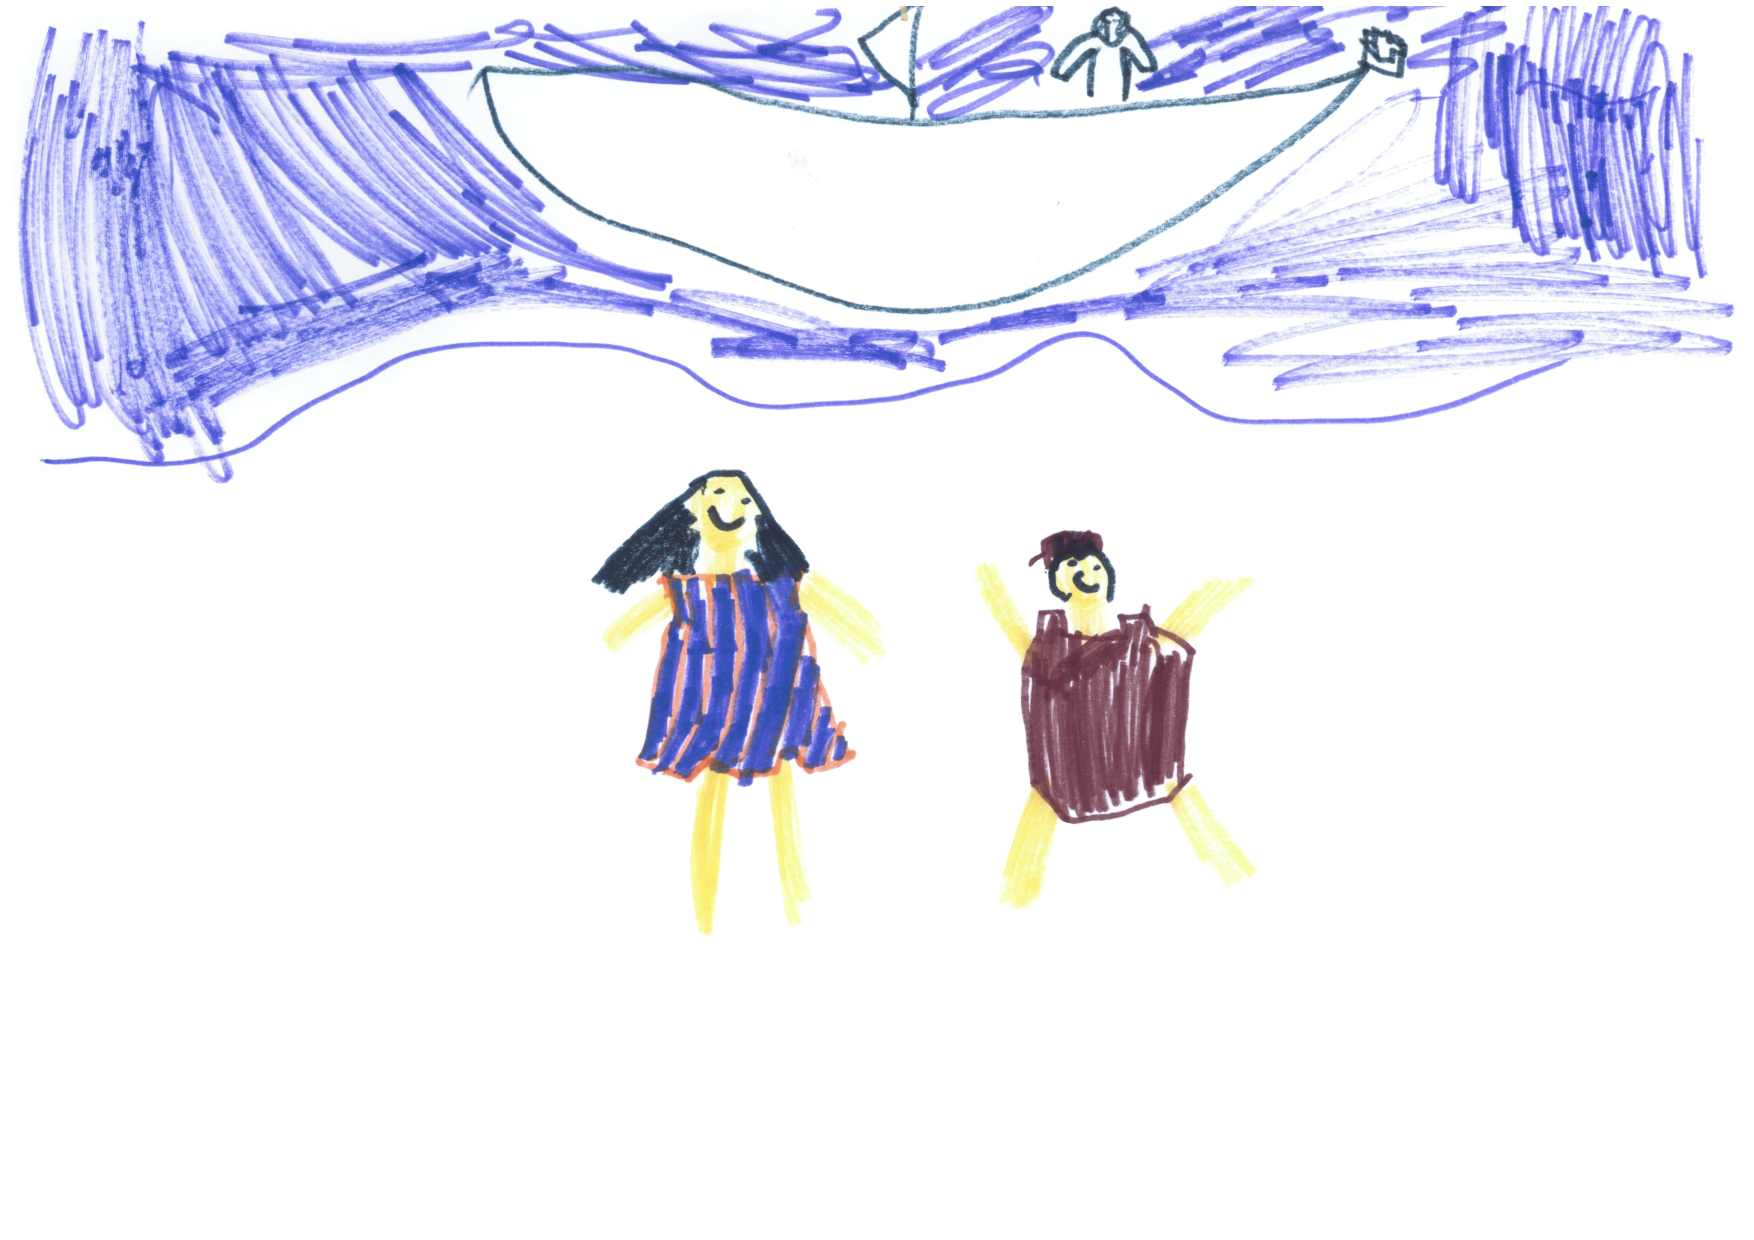
\includegraphics[width=.7\textwidth]{bilder/pirat1.pdf}
\end{figure}

Winnimon blickte fragend. Sie holte tief Luft und sagte: \enquote{Ich kann nicht fluchen. Mir fällt einfach kein Fluch ein. Du musst mir den besten Fluch verraten, den du kennst!}

\enquote{Aber warum willst du denn fluchen können?} Winnimon blickte fragend. \enquote{Du willst doch nicht etwa\dots?}

\enquote{Aber natürlich will ich auch Piratin werden! Meinst du ich will mein ganzes Leben hier verbringen? Ich will auch raus und die Welt sehen. Und jetzt hab ich dir geholfen, jetzt musst du mir helfen!}

Winnimon sah das sofort ein. Ihm ging es ja genauso. Und er zögerte nicht lange und verriet Drude seinen Lieblingsfluch. Das war er ihr schuldig, da gab es keine Frage. Ihm würde schon etwas einfallen.

Als beide zurück im Dorf waren, merkten sie gleich, dass etwas nicht stimmt. Vorbei am Haus von Winnimon sahen sie es auch schon. Ihm Hafen waren riesige Segel zu sehen und ganz oben auf dem höchsten Masten wehte die schwarze Fahne mit dem Totenkopf. Die Piraten waren da!

Sofort liefen die beiden hinunter zum Hafen. Das ganze Dorf hatte sich schon versammelt. Ein dicker Pirat stand in der Mitte der Menschenmenge auf einem Fass und rief:

\enquote{Liebe Leute. Mein Name ist Francisco San. Ich diene unter Barnabas Rotwild als erster Leutnant auf der Drachenblume, dem grössten Piratenschiff weit und breit. Wir sind gekommen, um zu fragen, ob jemand hier an Bord anheuern will. Wir nehmen zwei Schiffsjungen auf. Kommt mit uns, lernt die Welt kennen und werdet reich oder geht mit uns unter. Ihr alle kennt die drei Prüfungen. Aus all denen, die sie bestehen, nehmen wir zwei von euch auf. Freiwillige, tretet vor! Lang leben die Piraten!}

Alle Jungen und Mädchen waren sofort sehr aufgeregt, alle wollten mit. Nachdem sich die ersten getraut hatten vorzutreten, gaben sich auch Winnimon und Drude einen Ruck und stellten sich neben die anderen, alle in eine Reihe. Das alles so schnell gehen würde, hätten sie ja nie gedacht.

\enquote{Na dann wollen wir mal sehen.} Leutnant Francisco San schritt langsam die Reihe der Jugendlichen ab und zwirbelte dabei seinen Bart. \enquote{Ihr nehmt euch jetzt alle einen Stift und ein Stück Papier von dort drüben und schreibt folgende Wörter auf: Schatztruhe, Gewitter, arbeiten und Papagei.}

Die Prüfung war nur für zwei Jungen und ein Mädchen ein Problem, die ohne zu diskutieren den Stift hinlegten und aus der Reihe der Jugendlichen zurücktraten. Die waren schon durchgefallen. 

Bei der nächsten Prüfung, dem Fluchen, ging es sehr schnell zu. Jeder musste sich auf das Fass stellen und einmal so laut fluchen wie er konnte. 

\enquote{Dreibeiniger Hund}, \enquote{Vierauge}, \enquote{Vogelscheuche}, das waren so die Flüche die man hören konnte. Aber der Leutnant war nicht zufrieden. Die Flüche hätten alle schon einen längeren Bart als Kapitän Rotwild. Und wenn man so lange auf See ist und man immer die selben Flüche hört, wird einem echten Piraten sofort langweilig. Dann kamen Drude und Winnimon an die Reihe. Drude bestand den Test sofort mit mit dem {\it dreifach stinkenden Pups einer toten Ratte}. Sie war Winnimon sehr dankbar, denn mehr als Schwachkopf, aber da musste sie selbst zugeben, dass das sehr langweilig ist.

Winnimon brachte erst kein Wort heraus. So lange hatte er sich darauf verlassen, einen prima Fluch zu haben, dass er sich keinen neuen überlegt hatt. Wie angewurzrlt stand er auf dem Fass, aber dann brach es aus ihm heraus:

\enquote{Eitrige Warze am Bauch einer toten Ratte}. Der Leutnant lachte und sagte bestanden.

Danach waren nur noch drei Jugendliche im Rennen. Drude, Winnimon und ein weiterer Junge. Einer von denen die immer über Winnimon gelacht hatte, wenn der versucht hatte zu schwimmen. Er fühlte sich deswegen auch schon siegessicher, sprang gleich ins Meer, schwamm ein paar Züge und kam mit triumphierenden Lachen wieder aus dem Wasser. Drude machte es ihm nach. Jetzt waren alle Augen auf Winnimon gerichtet. Der sprang aber nicht gleich ins Wasser, sondern kletterte erst auf das Schiff, stellte sich auf die Reeling und blickte nach unten. Das Wasser war jetzt doch viel weiter weg, als er gedacht hatte. 

Die anderen Jungen fingen schon an zu lachen, da sprang Winnimon im weiten Bogen und mit Kopf voran in die nächste Welle. Als er wieder hoch kam, hatte er zwar Wasser geschluckt, liess sich aber nichts anmerken und schwamm zurück an Land. Alle klatschten, damit hätte niemand gerechnet.

Nur der Leutnant war unzufrieden. \enquote{Wir wollten ja nur zwei mitnehmen.} sagte er. \enquote{Na gut, dann stelle ich jedem von euch eine Frage. Du}, und dabei zeigte er auf Winnimon, \enquote{Wie heisst unser Piratenschiff}.

\enquote{Drachenblume!} Das war leicht für Winnimon. Er hatte schon so oft von der berühmten Drachenblume reden hören, er wusste alles über dieses Schiff. 

\enquote{Und Du}, diemal zu dem Jungen gewand \enquote{Was für ein Schiffstyp ist die Drachenblume?} Der Junge wurde bleich und ganz verlegen. Er wusste es nicht.

\enquote{Eine Galeone} rief Drude. Na klar, Drude wusste eigentlich fast alles. Sie war die beste der Klasse gewesen. 

\enquote{Damit ist es entschieden!} rief der Leutnant. \enquote{Ihr beiden kommt mit! Und wie es der Piratenbrauch verlangt, geht ihr sofort an Bord. Ihr dürft euch nicht nochmals umdrehen und von niemandem verabschieden. Euer altes Leben ist vorbei, ihr seid jetzt Piraten an Bord der Drachenblume.}

Winnimon und Drude hatten Tränen in den Augen. Das war jetzt doch alles sehr schnell gegangen. Aber sie bleiben tapfer und drehten sich nicht nochmals um, als sie auf das Schiff gingen. Sie hörten nur wie die Dorfbewohner klatschten. Als sie das Schiff betraten, fingen die Piraten an, alte Piratenlieder zu singen.

\itshape{15 Mann auf eines Toten Truh'}

\itshape{Johoho und ne Buddel voll Rum}

\itshape{Versoffen und beim Teufel ist die ganze Crew}

\itshape{Johoho und ne Buddel voll Rum}
\normalshape
\section*{\center $\skull$ Die ersten Tage als Pirat $\skull$}




  \hfill {\color{red}\decofourleft}

%Inhaltsverzeichnis
\newpage
\tableofcontents

\end{document}



